\chapter{Introduction}
\label{ch:introduction}

% ============================================================
% LAB GUIDE — Introduction (Ch.1) should contain:
%   1.1 Motivation
%   1.2 Goals
%   1.3 Structure of the thesis ("The thesis is structured as follows.")
% Self-check: a reader who only reads this chapter should know the problem,
% what this work delivers, and where to find each piece in the rest of the thesis.
% ============================================================

\section{Motivation}
\label{sec:motivation}

Robotic receptionists have been tested in public places for more than two decades, beginning with the CMU Roboceptionist Valerie~\cite{gockley2005longterm} and continued in long deployments such as the Robovie field study in a Japanese shopping mall~\cite{kanda2010shoppingmall}.
These earlier systems showed that people accept humanoid robots in real settings, but the dialogue itself was limited to scripted exchanges and rigid command menus.
The language layer, not the embodiment, was the main bottleneck.

\begin{figure}[htbp]
    \centering
    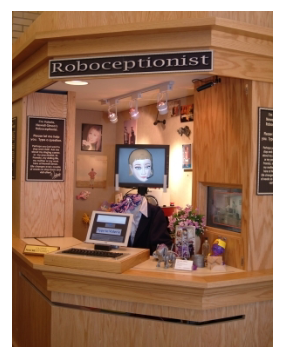
\includegraphics[width=0.55\textwidth]{src/figures/related_work/valerie.png}
    \caption{The CMU Roboceptionist Valerie, one of the earliest deployed receptionist robots~\cite{gockley2005longterm}.}
    \label{fig:valerie}
\end{figure}

Large language models (LLMs) change this picture by addressing the dialogue bottleneck that held the older systems back.
For a receptionist this is a big shift: a visitor can simply ask a question instead of choosing from a menu, and the robot can ground its reply in institutional information rather than giving a preprogrammed response.

Compared to a human at a reception desk, a robot offers some practical advantages.
It can work around the clock without breaks, hold a large and up-to-date set of facts about the building and the people in it, and does not get tired or impatient after the hundredth question of the day.
A human receptionist, of course, still has clear strengths: intuition, social judgment, and the ability to handle situations that the system has not been prepared for.
As the underlying technology improves this gap may narrow, but for now it remains real.


\section{Goals}
\label{sec:goals}

The goal of this thesis is to design an LLM-driven receptionist robot for social interaction, structured around the following eight tasks set by the thesis assignment:

\begin{enumerate}
    \item Review the related work on LLMs and social human--robot interaction (Chapter~\ref{ch:related_work}).
    \item Build a dialogue framework on Pepper that uses an LLM as its reasoning component (Chapter~\ref{ch:methods}).
    \item Add speech recognition and speech synthesis so the visitor can talk to the robot naturally.
    \item Add retrieval-augmented question answering so the robot can ground its replies in selected institutional documents.
    \item Add gestures that match what the robot is saying, and use Pepper's tablet to show useful information during the conversation.
    \item Try the full system in a receptionist-style scenario (Chapter~\ref{ch:experiments}).
    \item Compare a locally hosted LLM backend with a cloud-hosted backend in the same setup, to show the practical trade-offs of each approach.
    \item Evaluate the interaction using an established human--robot interaction questionnaire and feedback from visitors.
\end{enumerate}

\section{Structure of the Thesis}
\label{sec:thesis_structure}

% TODO (final pass before submission): re-read this section after every other
% chapter is finalised. The per-chapter summaries below can drift as content
% moves between chapters---make sure each sentence still matches what the
% chapter actually contains, drop anything that no longer applies, and check
% that no chapter has been added or removed without its preview being updated
% here.

The rest of the thesis is structured as follows.
Chapter~\ref{ch:related_work} reviews the related work: prior receptionist and guide robots, recent LLM-driven social robots, the role of gestures in human--robot interaction, and the questionnaire instruments used to evaluate social robots.
Chapter~\ref{ch:background} gives the conceptual background a reader needs to follow Chapter~\ref{ch:methods}: large language models and how their behavior is shaped through prompting, tool calling, and retrieval-augmented generation; speech interfaces for human--robot interaction; and the trade-offs between locally hosted and cloud-hosted LLM deployment.
Chapter~\ref{ch:methods} describes the system: the Pepper robot and the compute behind it, the service architecture, the two voice backends compared in this work (a locally hosted cascade and a cloud-hosted cascade), the knowledge-grounding layer that lets the robot answer questions about the institution, and the gesture and tablet feedback shown during the conversation.
Chapter~\ref{ch:experiments} presents the user study: the between-subjects design contrasting the two backends, the recruitment and procedure at the chosen reception desk, the questionnaire and custom items used to measure the interaction, and the objective, subjective, and qualitative results.
Chapter~\ref{ch:conclusion} gives a short summary of what was built and what was found.
Chapter~\ref{ch:discussion} discusses the limitations of the work and the implications of the results.
Chapter~\ref{ch:future_work} outlines directions for further work.

\begin{figure}[htbp]
    \centering
    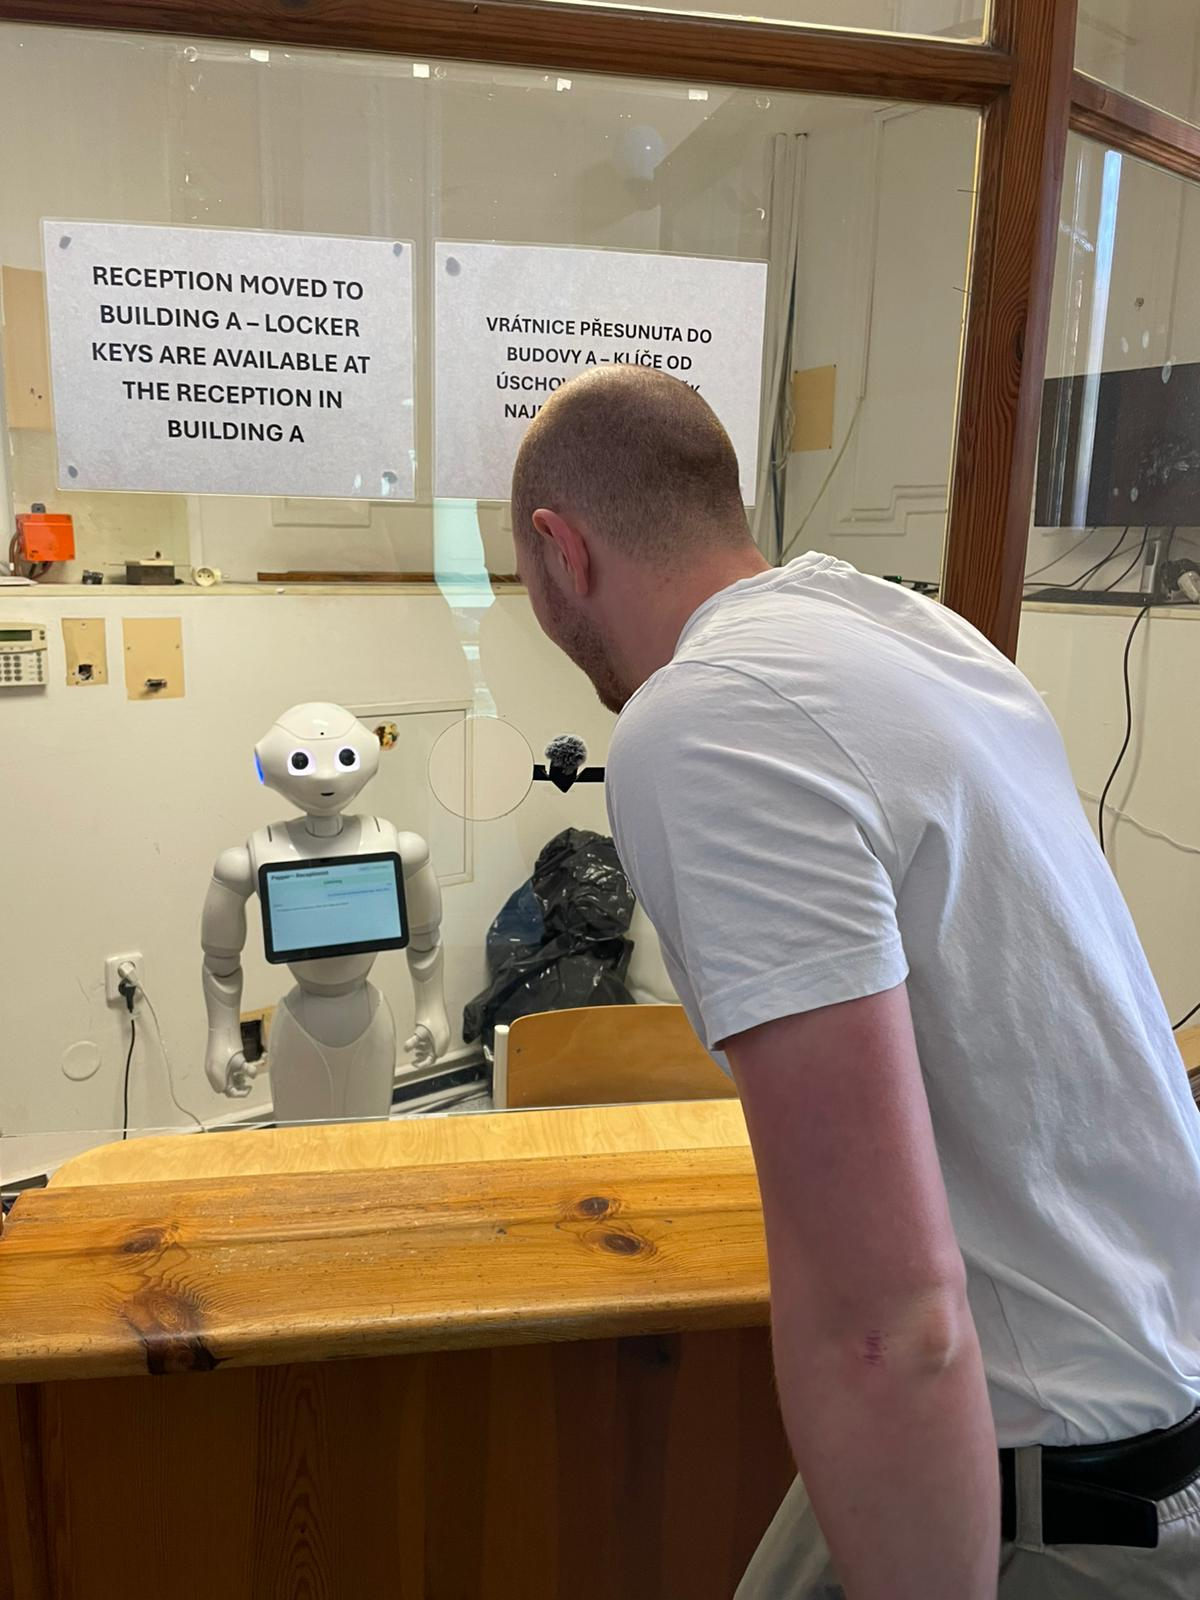
\includegraphics[width=0.5\textwidth]{src/figures/3rd_person.jpeg}
    \caption{The deployed system: a visitor talking to Pepper at the Building~E reception desk during the experiment.}
    \label{fig:third_person_intro}
\end{figure}
